\documentclass[12pt]{report}
\usepackage[utf8]{inputenc}
\usepackage[T1]{fontenc}
\usepackage{graphicx}
\usepackage{booktabs}
\usepackage{array}
\usepackage{enumitem}
\usepackage{hyperref}
\usepackage{geometry}
\geometry{a4paper, margin=1in}
\setcounter{secnumdepth}{3} % number sub-subsections (e.g. 2.1.1)

\begin{document}

\begin{center}

\includegraphics[width=2cm]{pes_logo.png} \\[0.5cm]
\textbf{\Large Dissertation on}\\[1cm]
\textbf{\Huge ``Adaptive Study Planning for\\ Self-Directed Learners''}\\[1cm]

Submitted in partial fulfilment of the requirements for the award of degree of\\[1cm]
\textbf{\Large Master of Technology in}\\[1cm]
\textbf{\Large Data Science}\\[1cm]
\textbf{Project Phase - 1}\\[1cm] % TODO: confirm course code for Phase 1

\textbf{Submitted by:}\\
\textbf{Rohit Saji}\\
\textbf{PES2PGXXDSXXX}\\[1cm] % TODO: registration number

Under the guidance of\\
Dr./Prof. [Guide Name]\\ % TODO: guide name
PES University\\[1cm]

January - June 2026\\[1cm] % TODO: confirm semester dates

DEPARTMENT OF COMPUTER SCIENCE AND ENGINEERING\\ % TODO: confirm department for DS programme
FACULTY OF ENGINEERING\\
PES UNIVERSITY\\[1cm]
(Established under Karnataka Act No. 16 of 2013)\\
Electronic City, Hosur Road, Bengaluru -- 560 100, Karnataka, India
\end{center}

\newpage

\section*{Certificate}

This is to certify that the dissertation entitled ``Adaptive Study Planning for Self-Directed Learners'' is a bonafide work carried out by \textbf{Rohit Saji (PES2PGXXDSXXX)} in partial fulfilment for the completion of Project Phase - 1 in the Program of Study -- Master of Technology in Data Science under the rules and regulations of PES University, Bengaluru.

\vspace{2cm}

\begin{flushright}
Dr./Prof. [Guide Name]\\ % TODO
PES University
\end{flushright}

\newpage

\section*{Declaration}

I hereby declare that the Project Phase - 1 entitled ``Adaptive Study Planning for Self-Directed Learners'' has been carried out under the guidance of Dr./Prof. [Guide Name], and submitted in partial fulfilment of the course requirements for the award of the degree of Master of Technology in Data Science of PES University, Bengaluru, during the academic semester January -- June 2026.

\newpage

\section*{Acknowledgement}

I would like to express my gratitude to my guide for continuous guidance and support throughout this project, and to the project coordinators for their help. I thank the Chairperson and faculty of the Department, PES University, for their support, and the university leadership for the opportunities provided. Finally, I extend heartfelt thanks to my family and friends for their constant encouragement.

\newpage

\section*{Abstract}

Self-directed learners routinely build fixed study plans that diverge from reality within days --- they fall behind or move ahead --- yet the plan never adapts, and learners have no reliable signal of how far off-track they are or whether they are genuinely learning. This work proposes an adaptive study-planning system that learns a learner's true pace, detects when their behaviour shifts, projects their completion date with calibrated uncertainty, and regenerates their schedule accordingly. The system is organised around two interlocking research pillars. The first, \textbf{closed-loop adaptation}, combines hierarchical Bayesian pace calibration, CUSUM change-point detection, and Gaussian-process progress projection with constraint-based schedule generation. The second, \textbf{assessment-based verification}, generates concept-tagged assessment items from the learner's own study material using large language models and applies cold-start knowledge tracing to estimate genuine concept mastery --- providing an honest learning signal that guards against unreliable self-reported study data and feeds verified estimates back into calibration. Candidate algorithms for each component are compared offline against established baselines on a literature-grounded synthetic dataset with known ground truth and on public knowledge-tracing benchmarks, using detection latency, interval calibration, AUC, and schedule-adherence metrics. Phase~I delivers and evaluates the open-loop system; Phase~II closes the loop and introduces assessment-based verification as the principal novelty, evaluated by comparing closed-loop adaptive planning against a static open-loop baseline on schedule adherence and measured learning gain. The expected contribution is a verified closed-loop study-planning system that integrates learner calibration, behavioural-shift detection, uncertainty-aware projection, and assessment-grounded verification for self-directed learners.

\newpage

\tableofcontents
\newpage
\listoffigures
\newpage
\listoftables
\newpage

\chapter{Introduction}

This chapter introduces the problem domain, the motivation for the project, the problem statement, the scope of the project, and the objectives to be achieved. It also provides an overview of the methodology followed and the structure of the report.

\section{Problem Statement}
Self-directed learners --- people working through online courses, exam preparation, or
self-study material without an instructor --- typically begin with a fixed study plan
(``two hours a day, finish by this date''). Within a few days the plan no longer matches
reality: the learner is ahead or behind, the plan does not adjust, and there is no
trustworthy signal of how far off-track they are or whether the time logged has produced
genuine learning. Existing tools either track time without planning, or generate static
plans that never adapt to the learner's realised pace, and none verify that self-reported
study actually resulted in learning.

\section{Objectives}
\begin{enumerate}[noitemsep]
    \item Learn a learner's true study pace from their own session history using
    hierarchical Bayesian calibration.
    \item Detect behavioural shifts in pace using statistical change-point detection.
    \item Project completion with calibrated uncertainty using Gaussian-process regression.
    \item Regenerate the study schedule using constraint-based, prerequisite-aware planning.
    \item Verify genuine learning by generating concept-tagged assessments from the
    learner's own material and estimating mastery via cold-start knowledge tracing,
    closing the loop by feeding verified mastery back into calibration.
    \item Evaluate the system against established baselines using synthetic data with
    known ground truth and public knowledge-tracing benchmarks.
\end{enumerate}

\section{Scope of the Project}
The project is delivered across two phases. \textbf{Phase~I} builds and evaluates the
open-loop system --- session logging, pace calibration, change detection, progress
projection, and static schedule generation --- and researches candidate approaches for
assessment-based verification. \textbf{Phase~II} closes the loop and implements the
chosen assessment-based verification approach as the principal novelty. The target user
is the individual self-directed learner; multi-user and institutional features are out of
scope.

\section{Organization of the Report}
Chapter~2 surveys related work across both research pillars and identifies the gaps.
Chapter~3 specifies system requirements. Chapter~4 describes the proposed methodology,
system architecture, algorithms, and expected outcomes. Chapters~5--7 cover
implementation, results, and conclusions, and are developed across the project phases.

\newpage

\chapter{Literature Survey}

This chapter surveys the research relevant to the project and identifies the gaps it
addresses. The work spans two research pillars, and the survey is organised accordingly.
Section~2.1 covers \textbf{Pillar~A --- adaptive pace modelling and scheduling}: learner
pace modelling and Bayesian calibration (\S2.1.1), behavioural-change detection
(\S2.1.2), progress prediction with Gaussian processes (\S2.1.3), adaptive scheduling and
study-plan generation (\S2.1.4), and self-regulated-learning analytics (\S2.1.5).
Section~2.2 covers \textbf{Pillar~B --- assessment generation, knowledge tracing, and
verification}: knowledge tracing and the cold-start problem (\S2.2.1), automatic
question generation with large language models (\S2.2.2), concept extraction and tagging
(\S2.2.3), automated answer evaluation (\S2.2.4), assessment integrity and gaming
detection (\S2.2.5), and retention and review scheduling (\S2.2.6). Section~2.3 summarises
the approaches in a comparison table, Section~2.4 lists the limitations of existing
systems, and Section~2.5 states the proposed solution.

\section{Existing Systems}

\subsection{Pillar A: Adaptive Pace Modelling and Scheduling}

\subsubsection{Learner Pace Modelling and Bayesian Calibration}
Estimating how fast a learner truly works, from limited per-learner data, is the
foundation of the adaptation pillar. Chen et al.~\cite{chen2024} propose a hierarchical
Bayesian model of adaptive teaching and validate it through two online behavioural
experiments with 312 adults, showing that hierarchical priors capture learner variability
without overfitting to sparse data --- the statistical justification for estimating a
single learner's pace from few sessions. Zanellati et al.~\cite{zanellati2024} present a
systematic review of hybrid knowledge-tracing models in the \textit{IEEE Transactions on
Learning Technologies}, building a taxonomy of approaches that combine Bayesian posteriors
with machine learning and concluding that hybrid models consistently outperform either
pure Bayesian Knowledge Tracing or pure deep learning. Zambrano et al.~\cite{zambrano2024}
analyse algorithmic bias in Bayesian Knowledge Tracing at scale and report that BKT
performance is essentially equal across demographic groups, supporting the reliable use of
BKT-family models across diverse learners. Complementing these, Mai et
al.~\cite{mai2025} propose a Transformer--Bayesian hybrid network that couples deep
temporal modelling with a probabilistic layer to recover interpretable, calibrated
knowledge estimates, reinforcing the finding that hybrid Bayesian designs retain
transparency without sacrificing predictive accuracy. These works establish Bayesian
calibration as sound for learner modelling but address correctness prediction rather than
the planned-versus-actual \emph{pace} estimation this project requires.

\subsubsection{Behavioural-Change Detection}
A learner's pace is not stationary; detecting when it shifts is essential to timely
replanning. Saqr et al.~\cite{saqr2026} apply critical-slowing-down (CSD) indicators in an
idiographic analysis of 1.67~million practice attempts from 9{,}401 students and find that
88.2\% of disengaging learners exhibit detectable warning signals beforehand --- strong
evidence that per-learner behavioural shifts are detectable from trace data. Qiao et
al.~\cite{qiao2026} provide a PRISMA systematic review of statistical-process-control
methods, documenting the mathematical rationale for CUSUM and EWMA control charts and
their machine-learning-enhanced variants, although all reviewed applications target
manufacturing rather than education. Boca de Giuli et al.~\cite{boca2024} combine control
charts with continual learning to distinguish endogenous system shifts from one-time
exogenous disruptions --- a distinction that maps directly onto the project's need to
recalibrate on genuine pace change while ignoring one-off disruptions. Closer to the
educational setting, Cheng et al.~\cite{cheng2024} model behavioural change directly from
heterogeneous student records --- assignments, grades, and attendance --- for early
at-risk prediction, deliberately retaining qualitative information that pure quantitative
feature extraction discards; this is evidence that behavioural-shift signals are
recoverable from the same kind of trace data this project logs. The gap is that these
methods detect shifts but prescribe no corrective action.

\subsubsection{Progress Prediction with Gaussian Processes}
Projecting a completion date \emph{with} a calibrated uncertainty band, rather than a
single number, is what makes a projection trustworthy. P\'erez-Suay et
al.~\cite{perezsuay2024} apply Gaussian-process (GP) regression with an
automatic-relevance-determination kernel to learning-management-system logs, achieving
$R = 0.89$ for predicting student marks with interpretable feature weighting. Chen and
Yao~\cite{chenyao2025} combine black-hole optimisation for feature selection with a
weighted GP-regression ensemble, reporting RMSE~$0.95$ and MAE~$0.81$ and showing that GP
predictions degrade gracefully with limited data. Lin et al.~\cite{lin2024} introduce a
latent Kronecker structure to scale GPs for learning-curve prediction, matching
Transformer performance while retaining calibrated uncertainty. Beyond regression,
Gaussian-process \emph{classification} with meta-heuristic hyper-parameter search has been
used to predict student performance bands~\cite{huang2025}, and integrated multi-modal
machine-learning frameworks report strong engagement- and dropout-prediction accuracy on
educational data~\cite{kayande2025} --- indicating that probabilistic and ensemble
predictors generalise across educational prediction tasks. These works validate GP
regression on educational data, but apply it cross-sectionally rather than to the
longitudinal burn-up projection the project needs.

\subsubsection{Adaptive Scheduling and Study-Plan Generation}
The system must turn estimates into a concrete, regenerated schedule. Islam et
al.~\cite{islam2024} couple an artificial neural network for grade prediction (accuracy
$\approx 0.73$) with dynamic programming for optimal schedule allocation, establishing the
\textit{predict-then-optimize} architecture this project adopts and extends; it is taken
as the base paper for Pillar~A. Fabregar and Amorado~\cite{fabregar2025} generate
expert-quality study plans in $0.32$~s using a greedy algorithm with prerequisite-constraint
satisfaction, demonstrating fast constraint-based, prerequisite-aware scheduling. Pagano
et al.~\cite{pagano2026} report a controlled study of 2{,}064 students showing that
adaptive learning paths produce substantial efficiency gains over static ones --- both
large-scale evidence that adaptation works and the template for an adaptive-versus-static
evaluation design. Knowledge-graph-based planners take a complementary route: Liu et
al.~\cite{liu2025} integrate a domain knowledge graph with AI-driven sequencing to generate
personalised learning paths that respect concept prerequisites, illustrating
prerequisite-aware path construction at the curriculum level. The limitation across these
works is that the generated plan is static: it never adapts to the learner's realised pace.

\subsubsection{Self-Regulated-Learning Analytics}
Alhazbi et al.~\cite{alhazbi2024} review 25 empirical studies on measuring self-regulated
learning (SRL) from trace data and find that most validated indicators relate to
time-management skills, grounding the project's choice of metrics --- schedule adherence
and regularity --- in established SRL frameworks. de Barba et al.~\cite{debarba2025}
develop and validate an SRL learning-analytics rubric that maps validated SRL scales onto
learning-management-system data indicators in a scalable, explainable way, providing a
template for turning raw trace data into interpretable self-regulation signals. Uzun et
al.~\cite{uzun2025} show empirically that learners' engagement with analytics feedback is
associated with both SRL competence and course performance, motivating the project's
feedback-oriented design. More broadly, hybrid machine-learning and rough-set models have
been applied to identify at-risk learners and trigger personalised
interventions~\cite{butt2025}, situating adherence analytics within a wider
student-management context. These works supply the validated indicators but stop at
measurement; none feeds the SRL signal back into an adaptive plan.

\subsection{Pillar B: Assessment Generation, Knowledge Tracing, and Verification}

\subsubsection{Knowledge Tracing and the Cold-Start Problem}
Knowledge tracing (KT) estimates a learner's evolving mastery from their response history
and is the mechanism this project uses to convert assessment outcomes into a verified
learning signal. The cold-start work of~\cite{clst2024} (CLST) observes that most KT models
are ID-based and perform poorly for new learners with little history, and mitigates this by
aligning a generative large language model as a student knowledge tracer; it is taken as
the base paper for Pillar~B because single-learner, few-session cold-start is precisely the
project's setting. MAML-KT~\cite{maml2026} frames new-student prediction as few-shot
model-agnostic meta-learning, showing that standard models (DKT, DKVMN, SAKT) exhibit
substantially lower early accuracy than reported once the cold-start scenario is made
explicit. DKVMN\&MRI~\cite{dkvmn2024} extends the Dynamic Key-Value Memory Network with
multi-relational information (exercise--knowledge-component and exercise--exercise
relations) to address sparse input and weak interpretability. Multi-concept modelling is
directly relevant here because assessment items rarely test a single concept: SLAM~\cite{slam2026}
models sequential learning signals across multiple concepts per question, relaxing the
single-concept assumption that limits many KT models, while~\cite{su2025} integrates
question-level information with learner behaviour to sharpen mastery estimates. The
concept-driven model
of~\cite{conceptkt2026} adds a \emph{personalised} forgetting mechanism, modelling
forgetting per learner and across related concepts rather than as a single time-decay ---
the closest prior work to this project's concept-level, retention-aware mastery model.
Graph-based KT for MOOC path recommendation~\cite{graphkt2025} models heterogeneous
relations among students, learning objects, and knowledge components and connects mastery
estimation to next-activity recommendation, bridging Pillar~B back to scheduling.

\subsubsection{Automatic Question and Item Generation with Large Language Models}
The verification pillar must first generate assessments from the learner's own material.
The systematic study of~\cite{itemgen2024} investigates LLM prompting for automatic item
generation across STEM subjects and characterises both the capability and the risks ---
hallucination and the promotion of misconceptions --- that any generation pipeline must
guard against. The self-hosted lecture-to-quiz pipeline of~\cite{lecturequiz2026} converts
lecture PDFs into multiple-choice questions using a \emph{local} LLM with deterministic
quality control, keeping content on-device and emitting auditable question banks; this is
close prior art for the project's ingest-material-to-assessment pipeline on a self-hosted
service. A growing body of work refines this capability for assessment specifically.
Nikolovski et al.~\cite{nikolovski2025} use LLM-based agents to align generated questions
with course objectives and Bloom's-taxonomy cognitive levels, improving clarity and
difficulty control. Recognising that fully automatic generation risks factual errors and
uneven difficulty, Burke~\cite{burke2025} proposes a human-in-the-loop framework for
exam-variant generation that retains template-level scalability while inserting expert
review, and Alamoudi et al.~\cite{alamoudi2025} combine LLMs with ontologies to optimise
automated question generation, reporting gains in semantic-similarity and BERT-based
quality metrics over flat-prompt baselines. Together these establish both the promise and
the quality-control discipline the project's generation pipeline must adopt.

\subsubsection{Concept and Knowledge-Component Extraction}
For knowledge tracing to operate over freshly generated items, each item must be tagged
with the concept it assesses. The work of~\cite{kctag2024} uses GPT-4 to generate and tag
knowledge components for multiple-choice questions in Chemistry and E-Learning and
validates them against three domain experts per subject, quantifying the
human--LLM discrepancy. Complementarily,~\cite{concepttag2024} automates knowledge-concept
tagging on mathematics questions using LLMs with a flexible demonstration retriever,
replacing manual expert annotation. Recent work frames this tagging as Q-matrix
construction: Lopes and Netto~\cite{qmatrix2026} evaluate LLM-generated
item--knowledge-component Q-matrices both structurally and functionally, treating the
matrix as an interpretable item--attribute mapping that a tracing model can consume
directly, and Hendrawan et al.~\cite{hendrawan2026} give a data-driven evaluation of
LLM-based ontology concept extraction from programming content, quantifying where automated
extraction succeeds and fails on the project's own domain. On the consuming side,
KeenKT~\cite{keenkt2026} disambiguates a learner's mastery state --- separating genuine
ability from an outburst or carelessness via a Normal-Inverse-Gaussian representation ---
which matters when mastery must be inferred from a small number of freshly generated items.
Together these establish the concept-tagging step that links generated items to the mastery
model.

\subsubsection{Automated Answer Evaluation and Grading}
Generated items must be graded automatically across the project's theory and coding
modalities. The work of~\cite{llmgrade2024} applies LLMs to grade open-ended short answers
in software-engineering courses, where many distinct answers may be partially correct,
demonstrating automated evaluation beyond pure code. The empirical study
of~\cite{essay2024} evaluates ChatGPT as an automated essay-scoring tool using
criteria-grounded prompts derived from the official TOEFL guide, situating LLM grading
against established deep-learning and statistical scoring methods. For the coding modality
specifically, Jukiewicz~\cite{jukiewicz2026} reports a large-scale, side-by-side comparison
of contemporary LLMs grading over 6{,}000 programming submissions, characterising the
consistency and leniency differences any automated coding-grader must account for. On the
theory side, rubric-grounded LLM grading of short answers~\cite{senanayake2024} and
comparative analyses of LLMs on open-ended mathematics responses~\cite{baral2024} confirm
that automated evaluation extends across free-text and numeric answers alike, while
underscoring the residual variability that argues for rubric anchoring and human
spot-checks.

\subsubsection{Assessment Integrity and Gaming Detection}
The motivation for verification is that self-reported activity can be gamed. The
think-aloud study of~\cite{gaming2026} analyses gaming the system through the lens of
self-regulated learning, moving beyond a purely behavioural view to ask whether students
are cognitively disengaged --- directly relevant to framing the ``fake session'' problem.
The multi-stage system of~\cite{integrity2024} detects online-assessment misconduct by
combining internet-protocol/geographical verification with behavioural analysis,
illustrating practical integrity safeguards for online assessment. Beyond protocol-level
checks, deep-learning and classical machine-learning models have been trained to flag
anomalous exam behaviour directly from interaction data~\cite{erdem2025}, demonstrating
data-driven cheating detection that complements the project's synthetic
honest-versus-faker evaluation.

\subsubsection{Retention and Review Scheduling}
Finally, the system must decide \emph{when} to assess. Personalised spaced-repetition
scheduling~\cite{spaced2025} schedules review at algorithmically chosen intervals to
maximise retention, informing the placement of assessments and reviews within the
generated roadmap; the personalised forgetting model of~\cite{conceptkt2026} provides the
complementary per-concept retention estimate. Closing the loop between generation and
retention, recent work uses LLMs to generate \emph{retrieval-practice} items scheduled at
spaced intervals~\cite{retrieval2025}, directly linking the project's two Pillar~B
capabilities --- item generation and review timing --- within a single retention-oriented
pipeline.

\subsection{Summary of Approaches}
Table~\ref{tab:litsummary} summarises the principal approach families across both pillars with
their strengths and the limitations that motivate this work. The recurring pattern is that
each technique is strong in isolation but disconnected from the others: none forms a
closed loop, and none uses assessment to verify the learning signal that drives planning.

\begin{table}[htbp]
\centering
\footnotesize
\caption{Summary of approach families across the two pillars, with strengths and limitations.}
\label{tab:litsummary}
\begin{tabular}{p{3.0cm} p{4.2cm} p{4.2cm}}
\toprule
\textbf{Approach family} & \textbf{Strengths} & \textbf{Limitations for this project} \\
\midrule
Bayesian calibration~\cite{chen2024,zanellati2024,zambrano2024,mai2025} & Works with sparse, per-learner data; interpretable; fair across groups & Targets correctness, not planned-vs-actual pace \\
Change-point detection~\cite{saqr2026,qiao2026,boca2024,cheng2024} & Detects behavioural shifts early; well-founded (SPC) & Detects only; prescribes no corrective replanning \\
Gaussian-process projection~\cite{perezsuay2024,chenyao2025,lin2024,huang2025,kayande2025} & Calibrated uncertainty; degrades gracefully with little data & Applied cross-sectionally, not to longitudinal burn-up \\
Adaptive scheduling~\cite{islam2024,fabregar2025,pagano2026,liu2025} & Fast, prerequisite-aware; adaptation shown to help & Generated plan is static; no feedback from realised pace \\
SRL analytics~\cite{alhazbi2024,debarba2025,uzun2025,butt2025} & Validated trace-based indicators of self-regulation & Measures behaviour; not tied to adaptive replanning \\
Knowledge tracing~\cite{clst2024,maml2026,dkvmn2024,conceptkt2026,graphkt2025,slam2026,su2025,keenkt2026} & Estimates mastery; cold-start and forgetting addressed & Assumes fixed item bank / many learners \\
LLM item generation~\cite{itemgen2024,lecturequiz2026,nikolovski2025,burke2025,alamoudi2025} & Generates assessments from raw material; self-hostable & Hallucination risk; decoupled from the learner's plan \\
Concept tagging~\cite{kctag2024,concepttag2024,qmatrix2026,hendrawan2026} & Automates KC linking of items & Studied apart from tracing and planning \\
Automated grading~\cite{llmgrade2024,essay2024,jukiewicz2026,senanayake2024,baral2024} & Scales evaluation across theory and code & Not connected to mastery estimation or scheduling \\
Integrity / gaming~\cite{gaming2026,integrity2024,erdem2025} & Surfaces dishonest engagement & Studied separately from planning \\
Retention scheduling~\cite{spaced2025,retrieval2025} & Times reviews to maximise retention & Not integrated with verified mastery \\
\bottomrule
\end{tabular}
\end{table}

\section{Limitations of Existing Systems}

\begin{enumerate}[noitemsep]
    \item \textbf{Techniques exist in isolation.} Calibration, change detection,
    projection, and scheduling are each studied alone; no system integrates them into a
    single connected loop.
    \item \textbf{No closed feedback to the schedule.} Behavioural monitoring~\cite{saqr2026}
    detects shifts but prescribes no corrective replanning; scheduling
    work~\cite{islam2024,fabregar2025} is static and does not adapt to realised pace.
    \item \textbf{No uncertainty-aware projection for self-directed learners.} GP
    work~\cite{perezsuay2024,lin2024} is cross-sectional; calibrated learning-curve
    projection is not applied to ongoing self-directed study.
    \item \textbf{Self-reported study activity is unverified.} No planning system uses
    assessment to confirm that logged study produced learning; gaming and self-report
    validity~\cite{gaming2026,integrity2024} are studied separately from planning.
    \item \textbf{Knowledge tracing assumes fixed item banks and many
    learners}~\cite{dkvmn2024,conceptkt2026}; even cold-start
    work~\cite{clst2024,maml2026} is not adapted to LLM-generated, per-learner,
    concept-tagged items in a single-learner setting.
    \item \textbf{Assessment generation, tagging, grading, and tracing are
    decoupled}~\cite{itemgen2024,lecturequiz2026,kctag2024,concepttag2024,llmgrade2024}
    from the learner's plan --- generated items are not used to drive calibration or
    rescheduling.
\end{enumerate}

\section{Proposed Solution}

This project proposes a \textbf{verified closed-loop} adaptive study-planning system for
self-directed learners, organised around two interlocking pillars that together close the
gaps above. \textbf{Pillar~A (closed-loop adaptation)} extends the predict-then-optimize
architecture~\cite{islam2024} into an adaptive loop: hierarchical Bayesian pace
calibration~\cite{chen2024}, change-point detection of behavioural
shifts~\cite{saqr2026,qiao2026}, Gaussian-process progress projection with calibrated
uncertainty~\cite{perezsuay2024}, and constraint-based, prerequisite-aware schedule
regeneration~\cite{fabregar2025}, evaluated with the adaptive-versus-static
paradigm~\cite{pagano2026} and self-regulated-learning metrics~\cite{alhazbi2024}.

\textbf{Pillar~B (assessment-based verification)} extends cold-start knowledge
tracing~\cite{clst2024,maml2026} to concept-level mastery over LLM-generated,
concept-tagged items~\cite{conceptkt2026,lecturequiz2026,kctag2024,concepttag2024}: the
system ingests the learner's own material, generates assessments~\cite{itemgen2024},
grades them~\cite{llmgrade2024}, and traces genuine mastery --- an honest learning signal
that guards against unverified self-reported study~\cite{gaming2026} and, in Phase~II,
feeds back into calibration to close the loop. Review placement draws on spaced-repetition
scheduling~\cite{spaced2025}. Phase~I delivers and evaluates the open-loop system; Phase~II
closes the loop and introduces assessment-based verification as the principal novelty ---
to the best of this survey's knowledge, the first study-planning system to integrate
learner calibration, behavioural-shift detection, uncertainty-aware projection, and
assessment-grounded verification for self-directed learners.

\newpage

\chapter{System Requirements Specification}

This chapter covers the system requirements, including hardware and software
specifications necessary for the project.

\section{Hardware Requirements}
\begin{itemize}[noitemsep]
    \item Commodity laptop/desktop (8~GB RAM or higher); no dedicated GPU required ---
    per-learner training data is small and models train on CPU.
    \item Local container runtime for the intelligence service (Docker via Colima).
\end{itemize}

\section{Software Requirements}
\begin{itemize}[noitemsep]
    \item \textbf{Client:} React + Vite (TypeScript), Dexie (IndexedDB) for local-first storage.
    \item \textbf{Intelligence service:} Python, FastAPI, Docker; scientific stack
    (NumPy, SciPy, scikit-learn) and knowledge-tracing tooling (pyKT, pyBKT).
    \item \textbf{Backend services:} Supabase (authentication, event database, storage).
    \item \textbf{External:} large-language-model API for assessment generation and grading.
\end{itemize}

\section{Functional Requirements}
The system shall log study sessions, calibrate learner pace, detect pace shifts, project
completion, generate and regenerate schedules, and (Phase~II) generate assessments and
estimate mastery.

\section{Non-Functional Requirements}
The core logging loop shall function offline; analytical results shall be cached locally;
the system shall scale to the individual-learner workload without specialised hardware.

\newpage

\chapter{Proposed Methodology}

This chapter explains the overall methodology, system architecture, algorithms, and the
expected outcomes against which the system will be evaluated.

\section{System Architecture}
The system follows a three-tier design (Figure~\ref{fig:architecture}): a local-first
client, a Python intelligence service that hosts all heavy machine-learning components,
and an offline research pipeline that produces the trained models the service runs.
Supabase acts as the data hub between client and service. Pillar~A (adaptation) runs as an
open loop in Phase~I; Pillar~B (verification) and the closed feedback loop --- in which
verified mastery is fed back into pace calibration --- are introduced in Phase~II.

\begin{figure}[p]
\centering
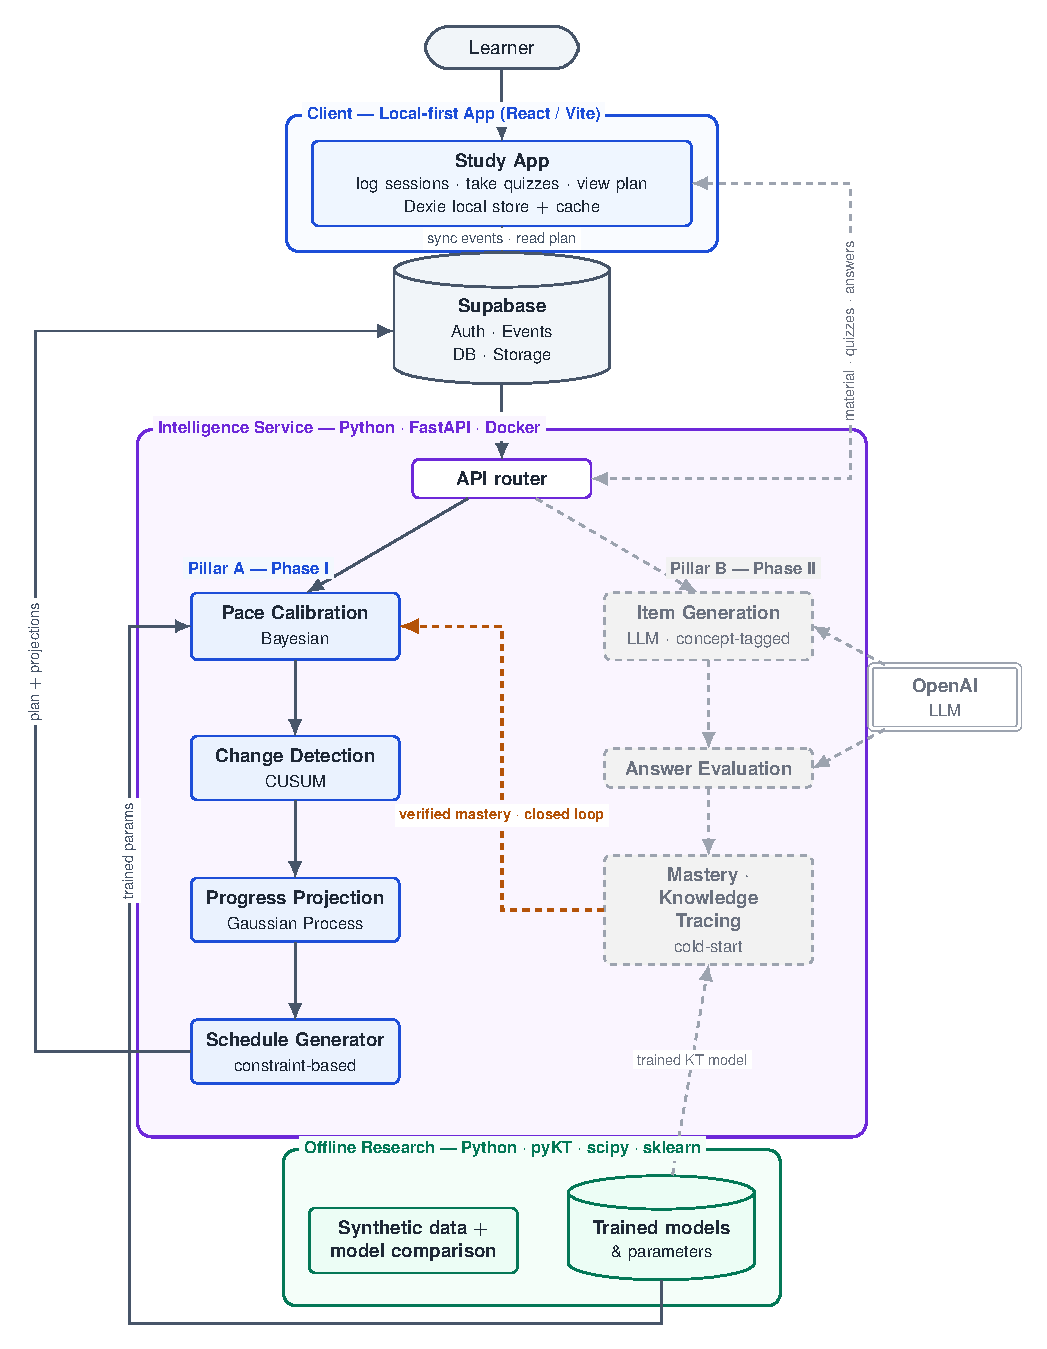
\includegraphics[width=0.82\textwidth]{system_architecture.pdf}
\caption{System architecture. Solid blue elements (Pillar~A: Bayesian pace calibration,
CUSUM change detection, Gaussian-process projection, constraint-based scheduling) run as an
open loop in Phase~I; dashed grey elements (Pillar~B: LLM item generation, answer
evaluation, cold-start knowledge tracing), the OpenAI dependency, and the verified-mastery
feedback edge are introduced in Phase~II. Supabase is the data hub; an offline research
pipeline supplies the trained models the engines run.}
\label{fig:architecture}
\end{figure}

\section{Algorithm and Model Description}
\textbf{Pillar~A} comprises four components: (i) hierarchical Bayesian \emph{pace
calibration} estimating the ratio of actual to planned effort at global, per-role, and
per-context levels; (ii) CUSUM \emph{change-point detection} over the pace-ratio time
series; (iii) Gaussian-process \emph{progress projection} producing a completion estimate
with a 95\% confidence interval; and (iv) constraint-based \emph{schedule generation} with
role-based material phasing. \textbf{Pillar~B} comprises (i) LLM-based \emph{item
generation} producing concept-tagged assessment items from ingested material;
(ii) \emph{answer evaluation} for theory and coding responses; and (iii) cold-start,
concept-level \emph{knowledge tracing} that estimates mastery and, in Phase~II, feeds the
verified signal back into calibration.

\section{Expected Outcomes and Evaluation Methodology}
Evaluation rests on three legs so that single-user data is not load-bearing:
(1)~\textbf{synthetic data with known ground truth} (planted pace, regime shifts, and
honest/faker labels) for precise algorithm comparison; (2)~\textbf{public benchmarks}
(knowledge-tracing datasets) for real-data credibility; and (3)~a \textbf{closed-loop
versus open-loop} comparison (Phase~II) with the candidate's own logged sessions as
longitudinal validation. Outcomes are stated as named metrics with directional
hypotheses; firm numbers follow once experiments are run.

\begin{table}[htbp]
\centering
\footnotesize
\caption{Expected outcomes --- Pillar~A (offline algorithm comparison).}
\label{tab:outcomes-a}
\begin{tabular}{p{2.3cm} p{3.1cm} p{3.0cm} p{4.0cm}}
\toprule
\textbf{Component} & \textbf{Metric} & \textbf{Compared against} & \textbf{Expected (directional)} \\
\midrule
Pace calibration & MAE / RMSE of predicted vs.\ actual pace & Hierarchical Bayesian vs.\ moving average & Bayesian lower error, especially with sparse data \\
Change detection & Detection latency, false-alarm rate & CUSUM vs.\ EWMA vs.\ CSD & A clear latency/false-alarm winner per profile \\
Progress projection & 95\% CI coverage, point error & Gaussian process vs.\ linear extrapolation & GP gives calibrated intervals; linear does not \\
Schedule generation & Deadline drift, schedule adherence & Constraint-based vs.\ rule-based vs.\ DP & Constraint-based competitive and prerequisite-aware \\
\bottomrule
\end{tabular}
\end{table}

\begin{table}[htbp]
\centering
\footnotesize
\caption{Expected outcomes --- Pillar~B (public benchmarks and synthetic honest/faker data).}
\label{tab:outcomes-b}
\begin{tabular}{p{2.3cm} p{3.1cm} p{3.0cm} p{4.0cm}}
\toprule
\textbf{Component} & \textbf{Metric} & \textbf{Compared against} & \textbf{Expected (directional)} \\
\midrule
Mastery model & AUC on public KT datasets & DKT, BKT baselines & Competitive AUC, $\approx 0.70$--$0.82$ (literature range) \\
Cold-start mastery & AUC at few interactions & Cold-start vs.\ standard KT & Cold-start higher AUC in low-data regime \\
Verification & Precision / recall of fake-session flags & Synthetic honest-vs-faker data & High precision without over-flagging honest learners \\
Item generation & Item validity / answerability rate & Human-checked sample & Majority valid; failure modes characterised \\
Learning signal & Pre/post mastery delta & --- & Detectable gain after genuine study \\
\bottomrule
\end{tabular}
\end{table}

\section{Workflow Diagram}
% TODO: add workflow figure if required.

\newpage

\chapter{Implementation Details}

This chapter provides details of the development process, programming languages, tools and
libraries, dataset descriptions, preprocessing, model building, and evaluation metrics.

\section{Development Environment}
% TODO

\section{Dataset Description}
% TODO: synthetic generator + public KT datasets (Eedi, POJ).

\section{Model Implementation}
% TODO

\section{Evaluation Metrics}
% TODO: see Chapter 4, Expected Outcomes.

\newpage

\chapter{Results and Discussion}

This chapter presents the experimental results obtained after testing the models,
including performance graphs, metric scores, and a comparative discussion with existing
methods.

\section{Result Analysis}
% TODO

\newpage

\chapter{Conclusion and Future Work}

This chapter summarizes the outcomes of the project, the conclusions drawn, and suggests
directions for future work.

\section{Conclusion}
% TODO

\section{Future Work}
% TODO: Phase II --- close the loop and implement assessment-based verification.

\newpage

\begin{thebibliography}{99}

\bibitem{islam2024} Islam, M., et al., ``Predicting Student Performance and Optimizing Study Schedule using Deep Learning and Dynamic Programming,'' \textit{Proc. International Conference on Computer and Information Technology (ICCIT)}, IEEE, 2024.

\bibitem{chen2024} Chen, et al., ``A Hierarchical Bayesian Model of Adaptive Teaching,'' \textit{Cognitive Science}, 2024.

\bibitem{zanellati2024} Zanellati, A., et al., ``Hybrid Models for Knowledge Tracing: A Systematic Review,'' \textit{IEEE Transactions on Learning Technologies}, 2024.

\bibitem{zambrano2024} Zambrano, A.~F., et al., ``Investigating Algorithmic Bias in Bayesian Knowledge Tracing,'' \textit{Proc. Learning Analytics and Knowledge (LAK)}, ACM, 2024.

\bibitem{saqr2026} Saqr, M., et al., ``Early Warning Signals Before Dropping Out: Critical Slowing Down Indicators,'' \textit{Proc. Learning Analytics and Knowledge (LAK)}, ACM, 2026.

\bibitem{qiao2026} Qiao, et al., ``Machine-Learning Approaches for Statistical Process Control: A Systematic Review,'' \textit{Entropy}, 2026.

\bibitem{boca2024} Boca de Giuli, et al., ``Monitoring and Continual Learning of Dynamical Models,'' \textit{Proc. European Control Conference (ECC)}, IEEE, 2024.

\bibitem{perezsuay2024} P\'erez-Suay, A., et al., ``Predicting Student Performance from Moodle Logs with Gaussian Processes,'' \textit{IEEE-RITA}, 2024.

\bibitem{chenyao2025} Chen, and Yao, ``Predicting Academic Achievement with Black-Hole-Optimized Gaussian Process Regression,'' \textit{Scientific Reports}, 2025.

\bibitem{lin2024} Lin, et al., ``Scaling Gaussian Processes for Learning-Curve Prediction with Latent Kronecker Structure,'' arXiv preprint, 2024.

\bibitem{pagano2026} Pagano, et al., ``Efficiency of Adaptive Learning Paths,'' \textit{Interactive Technology and Smart Education}, 2026.

\bibitem{fabregar2025} Fabregar, and Amorado, ``A Study Plan Recommender Based on a Greedy Algorithm,'' \textit{Proc. International Conference on Electrical Engineering and Informatics (EECSI)}, IEEE, 2025.

\bibitem{alhazbi2024} Alhazbi, S., et al., ``Using Learning Analytics to Measure Self-Regulated Learning: A Systematic Review,'' \textit{Journal of Computer Assisted Learning}, 2024.

\bibitem{mai2025} Mai, N.~T., Cao, W., Liu, W., ``Interpretable Knowledge Tracing via Transformer--Bayesian Hybrid Networks,'' \textit{Applied Sciences}, doi:10.3390/app15179605, 2025.

\bibitem{cheng2024} Cheng, J., Yang, Z.-Q., Cao, J., ``Modeling Behavior Change for Multi-model At-Risk Students Early Prediction,'' \textit{Proc. International Symposium on Educational Technology (ISET)}, IEEE, doi:10.1109/iset61814.2024.00020, 2024.

\bibitem{huang2025} Huang, K., Wang, C., ``A Gaussian Process Classifier Integrating Meta-Heuristic Optimisers to Predict Student Performance,'' \textit{International Journal of Information and Management Sciences}, doi:10.1504/ijims.2025.149393, 2025.

\bibitem{kayande2025} Kayande, D., Kukreja, S., ``An Integrated Multi-Modal Machine-Learning Framework for Real-Time Student Engagement Evaluation,'' \textit{MethodsX}, doi:10.1016/j.mex.2025.103588, 2025.

\bibitem{liu2025} Liu, X., Li, X., Chen, J., ``Adaptive Learning Path Planning System Based on Knowledge Graph and AI Integration,'' \textit{Proc. International Conference on Educational Technology (ICET)}, IEEE, doi:10.1109/icet67421.2025.11380560, 2025.

\bibitem{debarba2025} de Barba, P.~G., Oliveira, E.~A., English, N., ``Development and Validation of a Learning Analytics Rubric for Self-Regulated Learning,'' \textit{Educational Technology Research and Development}, doi:10.1007/s11423-025-10521-x, 2025.

\bibitem{uzun2025} Uzun, Y., Suraworachet, W., Zhou, Q., ``Engagement with Analytics Feedback and Its Relationship to Self-Regulated Learning Competence and Course Performance,'' \textit{International Journal of Educational Technology in Higher Education}, doi:10.1186/s41239-025-00515-3, 2025.

\bibitem{butt2025} Butt, A.~U.~R., Ali, H., Asif, M., ``Enhancing Student Management Through Hybrid Machine Learning and Rough Set Models,'' \textit{IEEE Access}, doi:10.1109/access.2025.3565585, 2025.

\bibitem{clst2024} ``CLST: Cold-Start Mitigation in Knowledge Tracing by Aligning a Generative Language Model as a Students' Knowledge Tracer,'' arXiv:2406.10296, 2024.

\bibitem{maml2026} ``MAML-KT: Addressing the Cold-Start Problem in Knowledge Tracing for New Students via Few-Shot Model-Agnostic Meta-Learning,'' arXiv:2603.00137, 2026.

\bibitem{dkvmn2024} ``DKVMN\&MRI: A New Deep Knowledge Tracing Model Based on DKVMN Incorporating Multi-Relational Information,'' \textit{PLoS ONE}, doi:10.1371/journal.pone.0312022, 2024.

\bibitem{conceptkt2026} ``Personalised Forgetting Mechanism with Concept-Driven Knowledge Tracing,'' doi:10.1145/3810940, 2026.

\bibitem{graphkt2025} ``Graph-based Knowledge Tracing for Personalized MOOC Path Recommendation,'' doi:10.69987/jacs.2025.51101, 2025.

\bibitem{itemgen2024} ``Automatic Item Generation in Various STEM Subjects Using Large Language Model Prompting,'' \textit{Computers and Education: Artificial Intelligence}, doi:10.1016/j.caeai.2024.100344, 2024.

\bibitem{lecturequiz2026} ``Self-hosted Lecture-to-Quiz: Local LLM MCQ Generation with Deterministic Quality Control,'' arXiv:2603.08729, 2026.

\bibitem{kctag2024} ``Automated Generation and Tagging of Knowledge Components from Multiple-Choice Questions,'' doi:10.1145/3657604.3662030, 2024.

\bibitem{concepttag2024} ``Automate Knowledge Concept Tagging on Math Questions with Large Language Models,'' arXiv:2403.17281, 2024.

\bibitem{llmgrade2024} ``Automatic Grading of Short Answers Using Large Language Models in Software Engineering Courses,'' \textit{Proc. EDUCON}, IEEE, doi:10.1109/educon60312.2024.10578839, 2024.

\bibitem{essay2024} ``Empirical Study of Large Language Models as Automated Essay-Scoring Tools in English Composition,'' arXiv:2401.03401, 2024.

\bibitem{gaming2026} ``Understanding Gaming the System by Analysing Self-Regulated Learning in Think-Aloud Protocols,'' doi:10.1145/3785022.3785025, 2026.

\bibitem{integrity2024} ``Advancing Online Assessment Integrity: Integrated Misconduct Detection via Internet-Protocol Analysis and Behavioural Analysis,'' \textit{IEEE Access}, doi:10.1109/access.2024.3434608, 2024.

\bibitem{spaced2025} ``Personalised Language Learning Using Spaced Repetition Scheduling,'' doi:10.1007/978-3-031-98459-4\_19, 2025.

\bibitem{slam2026} Jia, R., Jiang, Y.-H., Shen, Y., ``SLAM: Sequential Learning Signal Modeling for Multi-Concept Knowledge Tracing,'' \textit{Proc. IEEE International Conference on Acoustics, Speech and Signal Processing (ICASSP)}, doi:10.1109/icassp55912.2026.11464304, 2026.

\bibitem{su2025} Su, S., Zeng, P., Kang, C., ``Integrate Question Information With Learning Behavior for Knowledge Tracing,'' \textit{IEEE Access}, doi:10.1109/access.2025.3543536, 2025.

\bibitem{nikolovski2025} Nikolovski, V., Trajanov, D., Chorbev, I., ``Advancing AI in Higher Education: A Comparative Study of LLM-Based Agents for Exam Question Generation,'' \textit{Algorithms}, doi:10.3390/a18030144, 2025.

\bibitem{burke2025} Burke, C.~M., ``AI-Assisted Exam Variant Generation: A Human-in-the-Loop Framework for Automatic Item Creation,'' \textit{Education Sciences}, doi:10.3390/educsci15081029, 2025.

\bibitem{alamoudi2025} Alamoudi, S., Al Khuzayem, L.~A., Jamal, A., ``Optimizing Automated Question Generation for Educational Assessments,'' \textit{Engineering, Technology \& Applied Science Research (ETASR)}, doi:10.48084/etasr.10662, 2025.

\bibitem{qmatrix2026} Lopes, A.~M.~M., de Magalh\~aes Netto, J.~F., ``Large Language Models for Learning Technologies: Structural and Functional Evaluation of Automated Q-Matrix Generation,'' \textit{IEEE Access}, doi:10.1109/access.2026.3683811, 2026.

\bibitem{hendrawan2026} Hendrawan, R.~A., de Alencar, R.~S., Micheli, A., ``Data-Driven Evaluation of LLM-Based Ontology Concept Extraction from Programming Learning Content,'' \textit{Proc. Learning Analytics and Knowledge (LAK)}, ACM, doi:10.1145/3785022.3785106, 2026.

\bibitem{keenkt2026} Li, Z., Chen, L., Yi, J., ``KeenKT: Knowledge Mastery-State Disambiguation for Knowledge Tracing,'' \textit{Proc. AAAI Conference on Artificial Intelligence}, doi:10.1609/aaai.v40i23.39004, 2026.

\bibitem{jukiewicz2026} Jukiewicz, M., ``A Systematic Comparison of Large Language Models for Automated Assignment Assessment in Programming Education,'' \textit{Computers and Education Open}, doi:10.1016/j.caeo.2026.100364, 2026.

\bibitem{senanayake2024} Senanayake, C., Asanka, D., ``Rubric-Based Automated Short Answer Scoring Using Large Language Models,'' \textit{Proc. International Conference on Smart Computing and Systems Engineering (SCSE)}, IEEE, doi:10.1109/scse61872.2024.10550624, 2024.

\bibitem{baral2024} Baral, S., Worden, E., Lim, W.-C., ``Automated Assessment in Math Education: A Comparative Analysis of LLMs for Open-Ended Responses,'' \textit{Proc. Educational Data Mining (EDM)}, doi:10.5281/zenodo.12729932, 2024.

\bibitem{erdem2025} Erdem, B., Karabatak, M., ``Cheating Detection in Online Exams Using Deep Learning and Machine Learning,'' \textit{Applied Sciences}, doi:10.3390/app15010400, 2025.

\bibitem{retrieval2025} ``LLM-Generated Retrieval Practice: Linking Automatic Question Generation to Spaced Retrieval,'' arXiv:2507.05629, 2025.

\end{thebibliography}
\end{document}
